\chapter{\chapOne}
\label{cha:chapter1} % Label for hyperlink

% Start font-size
\begingroup
\fontsize{12pt}{14pt}\selectfont

\section{Einführung ins Thema}
Gestenerkennung und Gestensteuerung haben sich in den letzten Jahren von Nischenanwendungen im Gaming-Bereich, wie beispielsweise der Kinect-Plattform~\cite{Wiki:Kinect}, zu vielseitigen Steuerungsmöglichkeiten für virtuelle und reale Umgebungen entwickelt~\cite{RG:GestureRecognition}.
Ihre Wurzeln liegen teilweise in der Analyse der Gebärdensprache, reichen jedoch letztlich bis zu den Anfängen menschlicher Kommunikation zurück~\cite{Wiki:Gestenerkennung}\cite{RG:Gesten}.
Gesten stellen einen festen und wesentlichen Bestandteil der nonverbalen Verständigung dar und bilden somit eine natürliche Grundlage für intuitive Interaktionsformen zwischen Mensch und Maschine.~\cite[10]{Hobmair:Psy}

Parallel dazu gewinnt die autonome Steuerung technischer Systeme zunehmend an Bedeutung.
Fahrzeuge, die mit modernen Fahrassistenzsystemen ausgestattet sind, können heute vom Spurhalten bis zum automatischen Parkieren fast alles selbstständig ausführen.
Doch nicht nur im Strassenverkehr, auch in der Luft- und Schifffahrt werden Prozesse automatisiert, um Effizienz und Sicherheit zu erhöhen und menschliche Fehler zu minimieren.
Trotz dieser Entwicklungen bleibt der Mensch ein zentraler Bestandteil des Kontrollsystems: Er kann jederzeit in den automatisierten Ablauf eingreifen und die Steuerung übernehmen.~\cite{Wiki:aupi}

Noch rasanter schreitet die Entwicklung im Bereich der virtuellen und erweiterten Realität (VR und AR) voran~\cite{SD:VR}.
Hier ermöglichen innovative Interaktionskonzepte eine immer natürlichere, präzisere und intuitivere Steuerung digitaler Umgebungen.
Ein beeindruckendes Beispiel ist die Apple Vision Pro, eine VR-Brille, die im Jahr 2023 auf den Markt gekommen ist\textit{Apple Vision Pro}.
Das Gerät verfolgt die Bewegungen der Augen und verwendet diese als Gestensteuerung und erlaubt es, durch Zusammenführen von Daumen und Zeigefinger Objekte auf dem virtuellen Bildschirm auszuwählen.~\cite{apl:vision}

Auch in der Robotik eröffnen Gestensteuerungssysteme neue Perspektiven: Sie erlauben eine direkte, beinahe natürliche Kommunikation mit semi-autonomen oder autonomen Geräten, etwa bei der Navigation von Drohnen oder mobilen Robotern.
So können beispielsweise Bergungsarbeiten oder Minenräumungen künftig aus sicherer Entfernung durchgeführt werden, ohne dabei Menschen unnötigen Gefahren auszusetzen.

\section{Zielsetzung der Arbeit}
Das Ziel dieser Arbeit ist es, die Konzepte der Gestenerkennung sowie deren Einsatzmöglichkeiten zur Steuerung virtueller Systeme zu veranschaulichen.
Als Grundlage dient dabei ein ähnliches Projekt, das ein neuronales Netzwerk zur Erkennung von Handpositionen implementiert, um eine Steuerungsalternative zu traditionellen Kontrollern zu bieten.
Die Position der Hand wird von einer Kamera erfasst und von einem Computer ausgewertet.
Dieser sendet Steuerbefehle anhand der berechneten Daten an eine Renndrohne.~\cite{arxiv:OmniRace}

Um den Aufwand in einem realistischen Rahmen zu halten, wird in dieser Arbeit nicht auf eine direkte Erkennung der Fingerpositionen gesetzt.
Stattdessen kommen vier ArUco-Marker zum Einsatz, die auf der Steuerhand befestigt werden.
Dies soll eine präzise Erkennung der Handausrichtung ermöglichen, indem Flächen, Positionen und Distanzen der Marker berechnet und verglichen werden.
Anschliessend wird mit den in den \hTeLi{sec:cf}{Kapiteln~\ref{sec:cf}} und \hTeLi{sec:crpa}{\ref{sec:crpa}} beschriebenen Hardware-Komponenten eine Drohne gesteuert.

In diesem Projekt werden zwei Ansätze getestet, die sich in der Platzierung der Marker unterscheiden.
Der \hTeLi{pic:m1}{erste~Ansatz} sieht die Marker in einem Rechteck angeordnet vor, wobei ausschliesslich die Handfläche als Bereich für die Marker dient.
Der \hTeLi{pic:m2}{zweite~Ansatz} setzt hingegen drei von vier Markern auf den Fingerspitzen voraus.
Der vierte Marker wird auf dem Handgelenk platziert und markiert für die Kamera den Referenzpunkt der Hand.

\begin{figure}[H]
    \centering
    \begin{imgbox}
        \hspace{0.125\textwidth}
        \begin{subfigure}[b]{0.25\textwidth}
            \centering
            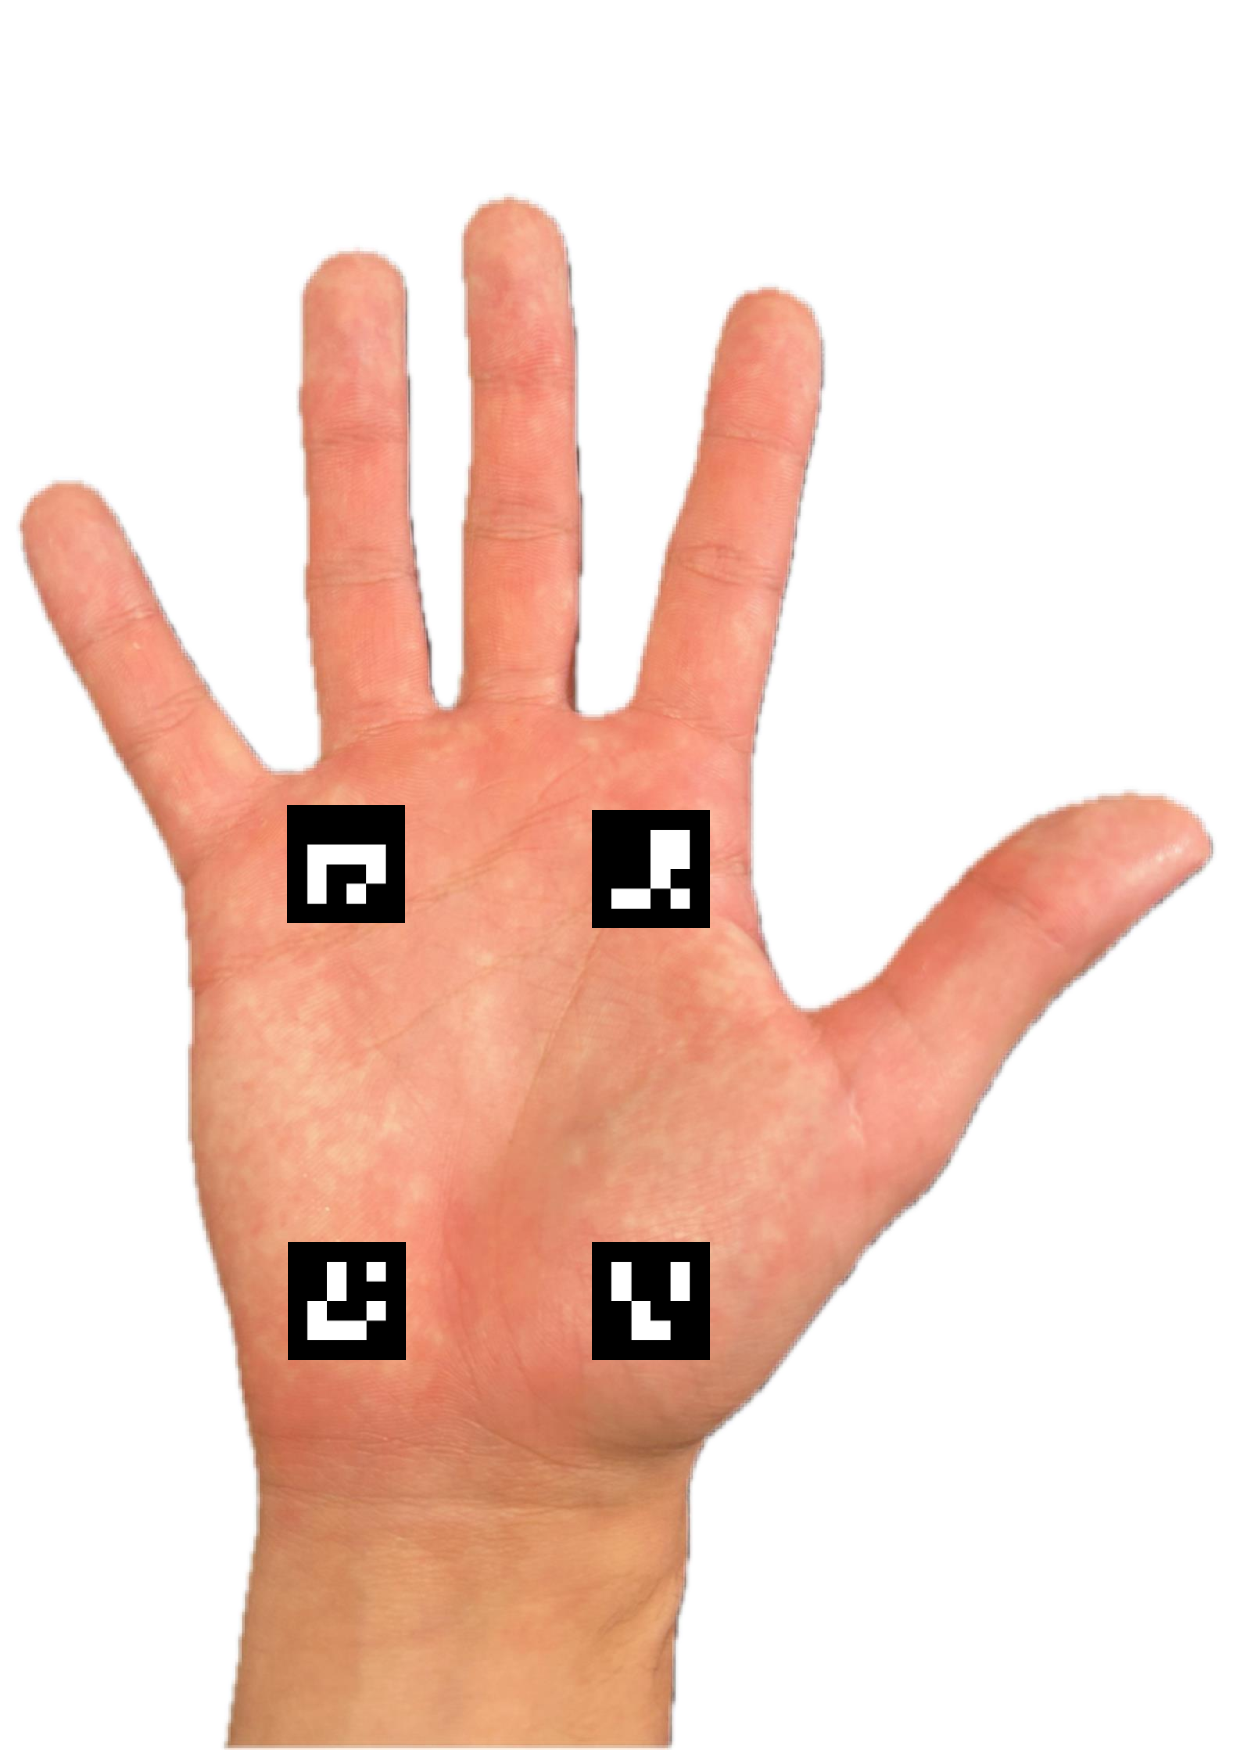
\includegraphics[width=\textwidth]{method1.pdf}
            \caption{Methode 1}
                \label{pic:m1}
        \end{subfigure}
        \hspace{0.125\textwidth}
        \vrule
        \hspace{0.125\textwidth}
        \begin{subfigure}[b]{0.25\textwidth}
            \centering
            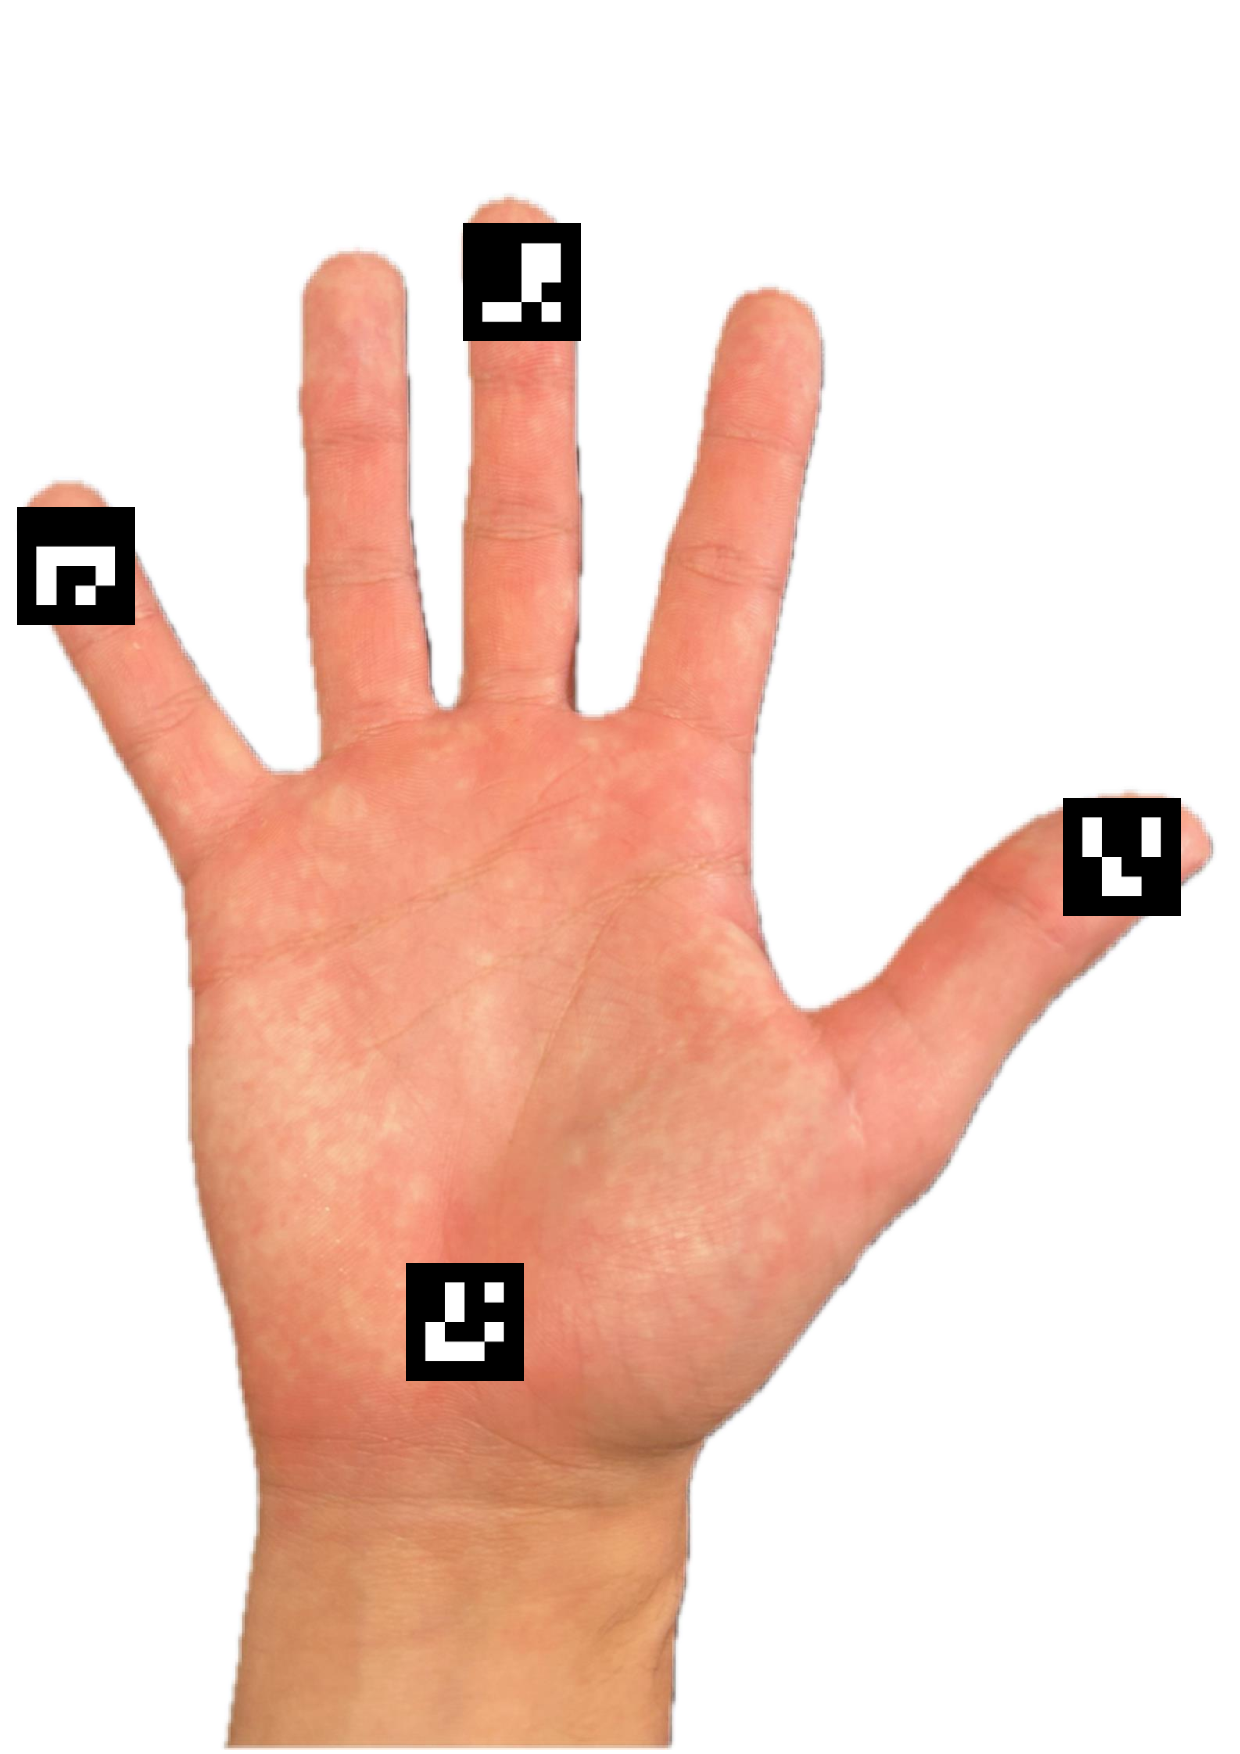
\includegraphics[width=\textwidth]{method2.pdf}
            \caption{Methode 2}
                \label{pic:m2}
        \end{subfigure}
        \hspace{0.125\textwidth}
    \end{imgbox}
    \caption{Ansätze}
        \label{fig:methods}
\end{figure}

Die unterschiedliche Platzierung der Marker soll zeigen, inwieweit die Einbeziehung der Finger die Erkennungsgenauigkeit und Steuerung beeinflusst.

\subsection{Prinzipielle Funktionsweise}
Im praktischen Einsatz bewegt der Benutzer seine Hand vor der Kamera, wobei die aufgeklebten ArUco-Marker erfasst und analysiert werden.
Welche Gesten dabei verwendet werden können und wie ihr Steuerbefehl lautet, ist im Folgenden aufgelistet:

\begin{itemize}
    \item \textbf{Neutral:} Die Handfläche ist Richtung Kamera und die Fingerspitzen noch oben ausgerichtet.
    \item \textbf{Vorwärts:} Handfläche ist maximal \SI{45}{\degree} mit der Handfläche in Richtung Kamera gebeugt.
    \item \textbf{Rückwärts:} Handfläche ist maximal \SI{45}{\degree} mit dem Handrücken in die entgegengesetzte Richtung der Kamera gebeugt.
    \item \textbf{Drehung nach rechts:} Neutrale Geste, aber nach rechts gedreht.
    \item \textbf{Drehung nach links:} Neutrale Geste, aber nach links gedreht.
    \item \textbf{Hoch:} Die Handfläche ist innerhalb des von der Kamera aufgenommenen Bildes eher oben.
    \item \textbf{Runter:} Die Handfläche ist innerhalb des von der Kamera aufgenommenen Bildes eher unten.
\end{itemize}

Aus den erkannten Positionen und Orientierungen werden Steuerbefehle abgeleitet, die über Funk an die Drohne gesendet werden.
Dadurch entsteht eine intuitive, gestenbasierte Steuerung, bei der die Ausrichtung der Hand unmittelbar die Flugbewegung der Drohne bestimmt.

\section{Forschungsgegenstand}
\subsection{Fragestellung, Hypothese}
Wie beeinflusst die Platzierung von ArUco-Markern auf der Hand die Genauigkeit und Zuverlässigkeit einer gestenbasierten Steuerung einer Nano-Drohne?  
Lässt sich durch die Einbeziehung der Finger in die Markeranordnung eine präzisere Erkennung der Handausrichtung und damit eine stabilere Steuerung erreichen?

Eine Markeranordnung, welche auch die Finger einbezieht, ermöglicht eine präzisere Bestimmung der Handausrichtung und führt somit zu einer zuverlässigeren und stabileren Steuerung der Drohne als eine ausschliesslich auf der Handfläche platzierte Markeranordnung.

\subsection{Abgrenzung (ausgeschlossene Faktoren)}
Im Rahmen dieses Projekts werden einige externe Einflussfaktoren bewusst ausgeklammert beziehungsweise nicht im Detail untersucht.
Dazu gehören insbesondere:
\begin{itemize}
  \item \textbf{Wind- und Luftströmungen:} Das System wird ausschliesslich in einer windstillen Indoor-Umgebung getestet.
  \item \textbf{Komplexe Handgesten:} Es wird davon ausgegangen, dass die ArUco-Tags jederzeit für die Kamera sichtbar bleiben.
  \item \textbf{Hindernisse und unebene Böden:} Die Testumgebung stellt ein Raum ohne potenzielle Hindernisse und mit matten, ebenen Böden dar.\footnotemark{}
\end{itemize}
\footnotetext{Der Grund dafür wir in \hTeLi{{sec:drco}}{Kapitel~\ref{sec:drco}} erklärt.}

% End font-size
\endgroup